%--------------------------------------------------------------------
\chapter{Probabilità sulla retta reale}
\setlength{\parindent}{2pt}

\begin{multicols*}{2}

Discutiamo in questa sezione la teoria della probabilità sulla
retta reale, uscendo dunque dal caso discreto. \smallskip

Per restringere la $\sigma$-algebra su cui lavoreremo (ossia l'insieme degli
eventi interessanti), siamo costretti a limitarci a una $\sigma$-algebra molto più
piccola di $\PP(\RR)$, la $\sigma$-algebra dei boreliani, che ci permette di escludere
``casi meno interessanti''. \smallskip

\begin{warn}
    Eccetto che nella prima sezione, assumeremo se non detto altrimenti
    di star lavorando sullo spazio misurabile
    $(\RR, \BB(\RR))$ dotato eventualmente della misura di Lebesgue $m$. $\BB(\RR)$ ed
    $m$ sono definiti nella sezione seguente.
\end{warn} 

\section{Cenni di teoria della misura}

\subsection{La \texorpdfstring{$\sigma$}{σ}-algebra di Borel e funzioni boreliane}

\begin{definition}[$\sigma$-algebra dei boreliani]
    Dato uno spazio metrico separabile\footnote{
        Si può generalizzare in modo naturale tale definizione a un qualsiasi spazio topologico.
        Dal momento che considereremo solo spazi metrici separabili (in particolare $X \subseteq \RR^d$), concentreremo
        le proprietà e le definizioni su questa classe di spazi topologici.} $X \neq \emptyset$
    si definisce la \textbf{$\sigma$-algebra $\BB(X)$ dei boreliani di $X$} (o
    $\sigma$-algebra di Borel)
    come la $\sigma$-algebra generata dai suoi aperti, ovverosia:
    \[
        \BB(X) \defeq \sigma \{ A \subseteq X \mid A \text{ aperto}\, \}.
    \]
    Gli elementi della $\sigma$-algebra di Borel sono detti \textit{boreliani}.
\end{definition}

\begin{proposition}[Proprietà di $\BB(X)$]
    Sia $X \neq \emptyset$ uno spazio metrico separabile. Allora valgono
    le seguenti affermazioni:

    \begin{enumerate}[(i.)]
        \item $\BB(X)$ contiene tutti gli aperti e i chiusi di $X$ (infatti
        metrico e separabile implica II-numerabile), pertanto se $\tau(X)$ è la
        topologia di $X$ vale che $\tau(X) \subseteq \BB(X)$,
        \item $\BB(X) = \sigma \{ A \subseteq X \mid A \text{ chiuso}\, \}$, ossia
        $\BB(X)$ è generata anche dai chiusi di $X$ (infatti $\BB(X)$ è chiuso per
        complementare),
        \item se $Y \subseteq X$, $Y \neq \emptyset$ ha metrica indotta da $X$, allora
        $\BB(Y) = \sigma \{ Y \cap B \mid B \in \BB(X) \} \subseteq \BB(X)$ (segue dal fatto che
        gli aperti di $Y$ sono tutti e solo gli aperti di $X$ intersecati a $Y$).
    \end{enumerate}
\end{proposition}

\begin{proposition}[Proprietà di $\BB(\RR^d)$]
    Valgono le seguenti affermazioni:
    \begin{enumerate}[(i.)]
        \item $\BB(\RR)$ contiene tutti gli intervalli e tutte le semirette (infatti si ammettono anche intersezioni infinite di aperti),
        \item $\BB(\RR)$ è generato dagli intervalli semiaperti, ovverosia $\BB(\RR) = \sigma \{ (a, b] \mid a, b \in \RR, a < b \}$,
        \item $\BB(\RR)$ è generato dalle semirette, ovverosia $\BB(\RR) = \sigma \{ (-\infty, a) \mid a \in \RR \}$,
        \item $\BB(\RR^d) = \sigma \{ (-\infty, a_1) \times \ldots \times (-\infty, a_n) \mid a_1, \ldots, a_n \in \RR \}$ (segue da (iii.)),
        \item $\BB(\RR^d) \neq \PP(\RR^d)$ (segue dal controesempio di Vitali, oltre che da considerazioni sulle cardinalità).
    \end{enumerate}
\end{proposition}

\begin{definition}[Funzione boreliana]
    Data una funzione $f : X \to Y$ con $X$ e $Y$ spazi metrici separabili, si dice che
    $f$ è una \textbf{funzione boreliana} se $f\inv(A)$ è boreliano per ogni
    $A$ boreliano di $Y$. Equivalentemente $f$ è boreliana se la controimmagine di ogni
    boreliano è un boreliano. \smallskip


    In particolare una funzione è boreliana se e solo se è misurabile rispetto
    alle $\sigma$-algebre di Borel.
\end{definition}

\begin{proposition}
    Sia $f : X \to Y$ con $X$ e $Y$ spazi metrici separabili una funzione continua. Allora
    $f$ è boreliana. \smallskip


    Segue dal fatto che $\BB(Y)$ è generato dagli aperti di $Y$, le cui controimmagini sono
    aperte, e dunque boreliane.
\end{proposition}

\subsection{Definizione e proprietà di misura, \texorpdfstring{$\pi$}{π}-sistemi per \texorpdfstring{$\sigma$}{σ}-algebre e lemma di Dynkin}

\begin{definition}[Misura]
    Dato $(\Omega, \FF)$ spazio misurabile, una misura $\mu$ su $(\Omega, \FF)$ è una
    funzione $\mu : \FF \to [0, \infty]$ con $\mu(\emptyset) = 0$ e per cui valga
    la $\sigma$-additività, ovverosia:
    \[
        \mu\left(\bigcupdot_{i \in \NN} A_i\right) = \sum_{i \in \NN} \mu(A_i), \quad A_i \in \FF.
    \]
\end{definition}

\begin{remark}[Proprietà basilari di una misura]
    Dal momento che si richiede per una misura valga $\mu(\emptyset) = 0$, si verifica
    facilemente che vale la $\sigma$-additività finita. \smallskip


    Inoltre, se $A \subseteq B$, allora $\mu(B) = \mu(B \setminus A \cupdot A) = \mu(B \setminus A) + \mu(A)$, e
    dunque vale sempre che $\mu(A) \leq \mu(B)$. Vale inoltre ancora la $\sigma$-subadditività, con la stessa
    dimostrazione data per la probabilità, e dunque:
    \[
        \mu\left(\bigcup_{i \in \NN} A_i\right) \leq \sum_{i \in \NN} \mu(A_i).
    \]
\end{remark}

\begin{remark}[Comportamento di $\mu$ al limite]
    Se $(A_i)_{i \in \NN}$ è una famiglia numerabile di
    insiemi in $\FF$, allora, seguendo la stessa dimostrazione
    data per le misure di probabilità, che:

    \begin{enumerate}[(i.)]
        \item $A_i \goesup A \implies \mu(A_i) \goesup \mu(A)$,
        \item $A_i \goesdown A \implies \mu(A_i) \goesdown \mu(A)$.
    \end{enumerate}
\end{remark}

\begin{definition}
    Una misura $\mu$ su $(\Omega, \FF)$ si dice \textbf{misura finita} se $\mu(\Omega)$ è finito.
\end{definition}

\begin{proposition}[Proprietà di una misura finita $\mu$]
    Sia $\mu$ una misura finita su $(\Omega, \FF)$. Allora valgono le seguenti affermazioni:
    \begin{enumerate}[(i.)]
        \item $P(A) = \frac{\mu(A)}{\mu(\Omega)}$ è una misura di probabilità,
        \item $\mu(A)$ è sempre finito e $\mu(\Omega) = \mu(A) + \mu(A^c)$,
        \item $A \subseteq B \implies \mu(B) = \mu(B \setminus A) + \mu(A)$,
        \item $\mu(B \setminus A) = \mu(B) - \mu(A \cap B)$,
        \item $\mu(A \cup B) = \mu(A \Delta B \cupdot A \cap B) = \mu(A) + \mu(B) - \mu(A \cap B)$,
        \item $\mu\left(\bigcup_{i \in [n]} A_i\right) = \sum_{j \in [n]} (-1)^{j+1} \sum_{1 \leq i_1 < \cdots < i_j \leq n} \mu\left(\bigcap_{k \in [j]} A_{i_{k}}\right)$ (Principio di inclusione-esclusione per le misure finite).
    \end{enumerate}

    Tutte le affermazioni seguono immediatamente dalla prima.
\end{proposition}

\begin{definition}[Insiemi $\mu$-trascurabili e proprietà che accadono $\mu$-quasi ovunque]
    Un insieme $A \in \FF$ si dice \textbf{$\mu$-trascurabile} se
    $\mu(A) = 0$. Una proprietà $M$ si dice che accade
    $\mu$-quasi ovunque ($\mu$-q.o.) se esiste $A \in \FF$ $\mu$-trascurabile per cui
    $M$ accade per $A^c$.
\end{definition}

\begin{definition}[\texorpdfstring{$\pi$}{π}-sistema di una $\sigma$-algebra]
    Sia $(\Omega, \FF)$ uno spazio misurabile. Allora un sottoinsieme $\mathcal{C} \subseteq \FF$
    si dice \textbf{$\pi$-sistema di $\FF$} se:
    \begin{enumerate}[(i.)]
        \item $A$, $B \in \mathcal{C} \implies A \cap B \in \mathcal{C}$ (chiusura per intersezioni),
        \item $\sigma(C) = \FF$ (genera $\FF$).
    \end{enumerate}
\end{definition}

\begin{remark}
    Un $\pi$-sistema contenente di una $\sigma$-algebra contenente $\Omega$ svolge lo ``stesso ruolo'' che una
    base svolge per una topologia.
\end{remark}

\begin{lemma}[di Dynkin, versione probabilistica]
    Sia $(\Omega, \FF)$ uno spazio misurabile e sia $\mathcal{C}$ un suo $\pi$-sistema contenente
    $\Omega$. Siano
    $P$ e $Q$ due probabilità sullo spazio misurabile di $\Omega$. Se $P$ e $Q$ coincidono su
    $\mathcal{C}$, allora $P \equiv Q$.
\end{lemma}

\begin{example}
    Alcuni esempi di $\pi$-sistemi contenenti $\RR$ per $(\RR, \BB(\RR))$ sono:
    \begin{itemize}
        \item gli aperti, ovverosia $\mathcal{C} = \{ A \in \FF \mid A \text{ aperto}\, \}$ (oppure i chiusi),
        \item le semirette (a sinistra), ovverosia $\mathcal{C} = \{ (-\infty, a] \mid a \in \RR \cup \{\infty\} \}$ (oppure le semirette a destra),
        \item gli intervalli semiaperti (a sinistra) con aggiunti $\emptyset$ e $\RR$, ovverosia $\mathcal{C} = \{ (a, b] \mid a, b \in \RR, b > a \} \cup \{\emptyset, \RR\}$ (oppure semiaperti a destra).
    \end{itemize}
\end{example}

\subsection{La misura di Lebesgue}

\begin{theorem}[Esistenza e unicità della misura di Lebesgue]
    Esiste ed è unica la misura $m$ su $(\RR, \BB(\RR))$ tale per cui
    $m([a, b]) = b-a$ per ogni $a$, $b \in \RR$ con $b > a$. Tale misura
    è detta \textbf{misura di Lebesgue} e corrisponde al concetto ``primitivo'' di
    \textit{lunghezza}. \smallskip


    L'unicità segue dall'enunciato generale del lemma di Dynkin.
\end{theorem}

\begin{remark}
    Dal momento che $m([0, 1]) = 1$,
    la misura $\restr{m}{[0,1]}$ è una misura di probabilità su $([0,1], \BB([0, 1]))$,
    detta \textit{probabilità uniforme su $[0,1]$}. Analogamente per $a$, $b \in \RR$
    con $b > a$, $m([a, b]) = b-a$ e
    dunque $P = \frac{1}{b-a} \restr{m}{[a,b]}$ è una misura di probabilità (detta
    \textit{probabilità uniforme su $[a,b]$}). \smallskip


    Assumendo l'assioma della scelta si può dimostrare che \underline{non} si può estendere in modo coerente
    $\restr{m}{[0,1]}$ a $([0, 1], \PP([0, 1]))$.
\end{remark}

\begin{remark}
    La misura di Lebesgue è nulla su un punto di $\RR$. Infatti, se $a \in \RR$, $m(\{a\}) =
    m([a-1, a] \cap [a, a+1]) = m([a-1, a]) + m([a, a+1]) - m([a-1, a] \cup [a, a+1]) =
    1 + 1 - m([a-1, a+1]) = 1 + 1 - 2 = 0$. Dunque, $m$ è in particolare nulla su insiemi
    numerabili (dacché si partizionano in modo numerabili sui punti). 
\end{remark}

\section{Probabilità reale, funzione di ripartizione (f.d.r.) e proprietà}

\subsection{Definizioni e proprietà della f.d.r.}

\begin{definition}
    Si dice \textbf{probabilità reale} una qualsiasi
    probabilità $P$ su $(\RR, \BB(\RR))$.
\end{definition}

\begin{definition}[Funzione di ripartizione di $P$]
    Data una probabilità reale $P$ si definisce
    allora la sua \textbf{funzione di ripartizione (f.d.r.)}
    come la funzione $F : \RR \to [0, 1]$ tale per cui:
    \[
        F(x) = P((-\infty, x]), \quad \forall x \in \RR.
    \]
    Si definisce inoltre $F(\pm\infty) \defeq \lim_{x \to \pm\infty} F(x)$.
    Indicheremo $F$ come $F_P$, e quando $P$ sarà nota dal contesto
    ci limiteremo a scrivere $F$.
\end{definition}

\begin{proposition}[Proprietà della f.d.r.]
    Sia $P$ una probabilità reale. Allora, se $F$ è la
    sua f.d.r.~vale che:
    \begin{enumerate}[(i.)]
        \item $F$ è crescente, ovvero $F(x) \geq F(y) \impliedby x \geq y$ (infatti $(-\infty, x] \supseteq (-\infty, y]$),
        \item $F$ è continua a destra, ovverosia per ogni $\tilde{x} \in \RR$ vale che $\lim_{x \to \tilde{x}^+} F(x) = F(\tilde{x})$,
        \item $F(-\infty) = 0 \impliedby ((-\infty, -i])_{i \in \NN} \goesdown \emptyset$,
        \item $F(\infty) = 1 \impliedby ((-\infty, i])_{i \in \NN} \goesup \RR$.
    \end{enumerate}


    L'affermazione (ii.)~segue dal fatto che per ogni successione decrecente da destra $(x_i)_{i \in \NN} \goesdown \tilde{x}$,
    che esclude $\tilde{x}$, è
    tale per cui $((-\infty, x_i])_{i \in \NN} \goesdown (-\infty, \tilde{x}]$, e dunque
    $(F(x_i))_{i \in \NN} = (P((-\infty, x_i]))_{i \in \NN} \goesdown P((-\infty, \tilde{x}]) = F(\tilde{x})$.
\end{proposition}

\subsection{Corrispondenza tra f.d.r.~e probabilità, calcolo di \texorpdfstring{$P$}{P} tramite \texorpdfstring{$F$}{F} e probabilità continue}

\begin{proposition}[$P$ è univocamente determinata da $F$]
    \label{prop:unicita_fdr}
    Sia $F : \RR \to \RR$ una funzione tale per cui:
    \begin{enumerate}[(i.)]
        \item $F$ è crescente,
        \item $F$ è continua a destra,
        \item $\lim_{x \to \infty} F(x) = 1$,
        \item $\lim_{x \to -\infty} F(x) = 0$.
    \end{enumerate}
    Allora $0 \leq F \leq 1$ ed esiste un'unica probabilità reale $P$ avente
    $F$ come funzione di ripartizione. \smallskip


    L'unicità segue dal lemma di Dynkin. Per l'esistenza è utile considerare
    che l'insieme delle discontinuità di $F$ è discreto dacché
    $F$ è crescente.
\end{proposition}

\begin{remark}
    La continuità a sinistra della f.d.r.~non è invece garantita dacché per ogni successione da sinistra crescente
    $(x_i)_{i \in \NN} \goesup \tilde{x}$, che esclude $\tilde{x}$,
    vale che $((-\infty, x_i])_{i \in \NN} \goesup (-\infty, \tilde{x})$, e non
    $(-\infty, \tilde{x}]$. Dunque $\lim_{x \to \tilde{x}^-} F(x)$ esiste ed è $P((-\infty, x))$, indicato
    comunemente come $F(x^-)$, che può non coincidere con $F(x)$. \smallskip

    Dal momento che:
    \[
        P(\{x\}) = P((-\infty, x] \setminus (-\infty, x)) = F(x) - F(x^-),
    \]
    si deduce che $F$ è continua se e solo se $P(\{x\}) = 0$ (ossia se e solo se
    $F(x) = F(x^-)$).
\end{remark}

\begin{remark}
    Si deducono immediatamente dalla precedente osservazione le seguenti identità:
    \begin{itemize}
        \item $P([a, b]) = F(b) - F(a^-)$,
        \item $P((a, b)) = F(b^-) - F(a)$,
        \item $P([a, b)) = F(b^-) - F(a^-)$,
        \item $P((a, b]) = F(b) - F(a)$.
    \end{itemize} 
\end{remark}

\begin{definition}[$P$ continua]
    Si dice che una probabilità reale $P$ è \textbf{continua} se
    la sua f.d.r.~$F$ lo è, ossia se $P(\{a\}) = 0$ per ogni $a \in \RR$
    (quest'ultima equivalenza deriva dalla penultima osservazione). 
\end{definition}

\begin{remark}
    Per una probabilità $P$ continua la misura di un intervallo con estremi $a$ e $b$ è semplificata
    a $F(b) - F(a)$ in tutti i casi (infatti $F(a^-) = F(a)$ e $F(b^-) = F(b)$).  
\end{remark}

\section{Classi principali di probabilità reale}

Esistono due classi importanti, ma non esaustive, di probabilità reale: le
probabilità discrete e quelle assolutamente
continue, contenute tra quelle continue. Le classi di probabilità reali
si dividono dunque secondo il seguente schema:

\begin{center}
    \tikzset{every picture/.style={line width=0.75pt}} %set default line width to 0.75pt        

    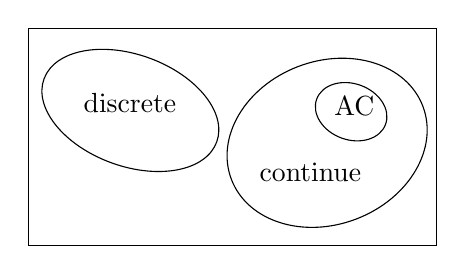
\begin{tikzpicture}[x=0.75pt,y=0.75pt,yscale=-1,xscale=1,scale=0.8]
    %uncomment if require: \path (0,300); %set diagram left start at 0, and has height of 300
    
    %Shape: Rectangle [id:dp7885262489349896] 
    \draw   (220.19,65.28) -- (466.19,65.28) -- (466.19,196.28) -- (220.19,196.28) -- cycle ;
    %Shape: Ellipse [id:dp8572353674963273] 
    \draw   (229.69,95.79) .. controls (236.04,78.39) and (264.48,72.78) .. (293.2,83.27) .. controls (321.92,93.76) and (340.05,116.37) .. (333.7,133.77) .. controls (327.34,151.17) and (298.91,156.78) .. (270.19,146.29) .. controls (241.47,135.8) and (223.33,113.19) .. (229.69,95.79) -- cycle ;
    %Shape: Ellipse [id:dp3583963732297444] 
    \draw   (342.58,156.41) .. controls (332.85,131.07) and (350.75,100.63) .. (382.58,88.41) .. controls (414.4,76.19) and (448.08,86.82) .. (457.81,112.15) .. controls (467.54,137.48) and (449.63,167.93) .. (417.81,180.15) .. controls (385.99,192.37) and (352.31,181.74) .. (342.58,156.41) -- cycle ;
    %Shape: Ellipse [id:dp5413476700533957] 
    \draw   (393.91,107.98) .. controls (397.1,99.22) and (408.98,95.52) .. (420.44,99.7) .. controls (431.9,103.89) and (438.6,114.38) .. (435.4,123.13) .. controls (432.21,131.89) and (420.33,135.59) .. (408.87,131.41) .. controls (397.41,127.22) and (390.71,116.73) .. (393.91,107.98) -- cycle ;
    
    % Text Node
    \draw (252,103) node [anchor=north west][inner sep=0.75pt]   [align=left] {discrete};
    % Text Node
    \draw (358,145) node [anchor=north west][inner sep=0.75pt]   [align=left] {continue};
    % Text Node
    \draw (403,105) node [anchor=north west][inner sep=0.75pt]   [align=left] {AC};
    \end{tikzpicture}
\end{center}

\begin{example}[Esempio di probabilità né discreta né continua]
    Sia $F : \RR \to \RR$ tale per cui:
    \[
        F(x) = \begin{cases}
            0 & \text{se } x < 0, \\
            x + \frac{1}{2} & \text{se } 0 \leq x \leq \frac{1}{2}, \\
            1 & \text{altrimenti}.
        \end{cases}
    \]
    Allora $F$ è crescente, continua a destra e tale per cui
    $\lim_{x \to -\infty} F(x) = 0$, $\lim_{x \to \infty} F(x) = 1$.
    Pertanto esiste un'unica probabilità $P$ avente $F$ come f.d.r.~per la
    \textit{Proposizione \ref{prop:unicita_fdr}}. \smallskip


    Dal momento che $F$ non è continua a sinistra in $0$, $F$ non è continua, e dunque
    $P$ non è continua. Inoltre $F$ non induce una probabilità discreta dacché
    non è costante a tratti in $[0, \nicefrac{1}{2}]$. Pertanto $P$ non è né
    continua né discreta.
\end{example}

\section{Probabilità discreta e rappresentazione della f.d.r.}

Come già discusso nella sezione della \textit{\hyperref[sec:discretizzazione]{Discretizzazione}},
una probabilità reale $P$ si dice \textit{discreta} se esiste $\Omega_0 \subseteq \RR$
discreto per cui $P$ è concentrata su $\Omega_0$. In tal caso, come già visto,
$P(A) = P(A \cap \Omega_0)$ per ogni $A \in \BB(\RR)$, e dunque $P$ è univocamente determinata
dalla densità discreta di $\restr{P}{\PP(\Omega_0)}$, che chiameremo $p$. \smallskip


In questo caso il range $R_P$ è dunque numerabile e, se $F$ è la f.d.r.~di $P$, vale che:
\[
    F(x) = P((-\infty, x]) = \sum_{\substack{y \in R_P \\ y \leq x}} p(y).
\]

\begin{remark}
    Se $P$ è discreta, come già osservato nella sezione della \textit{\hyperref[remark:identità_discreta_dirac]{Discretizzazione}},
    allora vale che:
    \[
        P = \sum_{x \in R_P} p(x) \, \delta_x.
    \]
\end{remark}

\begin{remark}
    Se $R_P$ non ha punti di accumulazione, allora $F$ è costante a tratti con salti
    negli $y \in R_P$ di ampiezza $p(y)$. \smallskip


    Al contrario, presa una successione $(p_r)_{r \in \QQ}$ con $\sum_{r \in \QQ} p_r = 1$,
    la probabilità $P = \sum_{r \in \QQ} p_r \, \delta_r$ è una probabilità discreta con
    f.d.r.~non costante a tratti (infatti tutti i punti di $\QQ$ sono punti di accumulazione). 
\end{remark}

Pertanto, se una probabilità reale è discreta, ci si può effettivamente restringere a tutti
i risultati della \textit{Parte 2}.

\section{Probabilità assolutamente continue (AC)}

\begin{warn}
    Si ricorda che con il simbolo $\int$ si intende l'integrale
    secondo Lebesgue e che si assume di star lavorando sempre con la
    misura di Lebesgue $m$.
\end{warn}

\subsection{Probabilità AC e funzione di densità}

\begin{definition}[Probabilità assolutamente continua (AC) e densità]
    Una probabilità $P$ si dice \textbf{assolutamente continua (AC)}
    se esiste una funzione
    boreliana $f : \RR \to \RR$ tale per cui:
    \[
        P(A) = \int_A f(x) \dx,
    \]
    dove si impiega l'integrale secondo Lebesgue. Tale funzione $f$ è
    detta \textbf{densità} di $P$. \smallskip


    Si assume implicitamente che $\int_\RR \abs{f(x)} \dx$ sia finito.
\end{definition}

\begin{remark}
    Se $P$ è AC, allora la sua f.d.r.~$F$ è in particolare
    assolutamente continua, e dunque anche continua.
\end{remark}

\begin{remark}
    Nella pratica l'integrale $\int_A f(x) \dx$ si riduce in molti casi
    al più semplice integrale di Riemann, eventualmente improprio.
\end{remark}

\subsection{Proprietà e caratterizzazione della densità}

\begin{proposition}[Unicità della densità a meno di $m$-trascurabilità]
    Se $P$ è una probabilità AC con densità $f$ e $g$, allora
    $f = g$ q.o.~(e dunque $m(f \neq g) = 0$, ossia l'insieme
    $f \neq g$ è $m$-trascurabile).
\end{proposition}

\begin{remark}
    Si osserva che se $P$ è una probabilità AC con densità
    $f$, allora $f \geq 0$ q.o.~per continuità (altrimenti $P$ potrebbe
    assumere valori negativi) e $\int_\RR f(x) \dx = P(\RR) = 1$.
\end{remark}

\begin{proposition}[La densità determina univocamente la probabilità]
    Sia $f : \RR \to \RR$ una funzione boreliana tale per cui:
    \begin{enumerate}[(i.)]
        \item $f \geq 0$,
        \item $\int_\RR f(x) \dx = 1$.
    \end{enumerate}
    Allora esiste un'unica probabilità reale $P$ avente $f$ come densità.
\end{proposition}

\begin{proposition}[Relazioni tra la densità e la f.d.r.]
    Sia $P$ una probabilità reale con f.d.r.~$F$. Allora valgono le seguenti affermazioni:
    \begin{enumerate}[(i.)]
        \item Se $P$ è AC con densità $f$, allora $F(x) = \int_{-\infty}^x f(y) \dy$. Viceversa
        se esiste $f$ per cui $F(x) = \int_{-\infty}^x f(y) \dy$, allora $P$ è AC con densità
        $f$.
        \item Se $F$ è continua e $C^1$ a tratti (ovverosia si restringe a una funzione $C^1$ eccetto che per un insieme di punti isolati),
        allora $P$ è AC con densità $f$ t.c.~$f = F'$ dove è definibile $F'$ e $f = 0$ altrimenti (segue dal Teorema fondamentale del calcolo integrale).
    \end{enumerate}
\end{proposition}

\begin{remark}
    Se $P$ è AC con densità $f$, allora $P(f = 0) = \int_{f = 0} f(x) \dx = 0$ e dunque
    l'insieme $f = 0$ è trascurabile rispetto a $P$. Dunque, ristringendo il range si
    ottiene che:
    \[
        P(A) = P(A \cap (f > 0)).
    \]
\end{remark}

\section{Variabili aleatorie in generale}

In questa sezione cerchiamo di generalizzare il concetto di variabile aleatoria
al caso più generale usando il linguaggio delle $\sigma$-algebre e delle
funzioni misurabili in modo tale da estendere coerentemente le v.a.~discrete.

\subsection{Definizione e legge di una v.a.}

\begin{definition}[Variabile aleatoria]
    Sia $(\Omega, \FF, P)$ uno spazio di probabilità. Allora, se
    $(S, \cS)$ è uno spazio misurabile e $X$ è una funzione misurabile
    da $\Omega$ a $S$, allora si dice che $X$ è una \textbf{variabile aleatoria (v.a.)}.
    Se $S = \RR$ e $\cS = \BB(\RR)$, si dice che $X$ è una \textit{v.a.~reale},
    se $S = \RR^d$ e $\cS = \BB(\RR^d)$, si dice che $X$ è una \textit{v.a.~vettoriale}
    o \textit{vettore aleatorio}.
\end{definition}

\begin{remark}
    Se $\Omega$ è discreto, $\FF = \PP(\Omega)$, e dunque ogni funzione
    $X : \Omega \to S$ è una variabile aleatoria. Pertanto la definizione
    espressa è una perfetta estensione del concetto di v.a.~discreta.
\end{remark}

\begin{definition}[Legge di $X$]
    Sia $(\Omega, \FF, P)$ uno spazio di probabilità e sia
    $X : (\Omega, \FF) \to (S, \cS)$ una v.a. Allora si dice
    \textbf{legge di $X$} (o \textit{distribuzione}) la probabilità
    su $P^X$ su $(S, \cS)$ tale per cui:
    \[
        P^X(A) = P(X \in A) = P(X\inv(A)).
    \]
\end{definition}

\subsection{F.d.r.~di una v.a.~reale, v.a.~discrete, continue e AC}

\begin{definition}[F.d.r.~di una v.a.~reale]
    Si definisce la \textbf{funzione di ripartizione (f.d.r.) di una
    v.a.~$X$} come la f.d.r.~$F^X$ associata alla probabilità reale
    $P^X$, ovverosia:
    \[
        F^X(x) = P(X\inv((-\infty, x])) = P(X \leq x).
    \]
\end{definition}

\begin{definition}[V.a.~discreta]
    Una v.a.~$X : \Omega \to S$ si dice \textbf{discreta} se
    la probabilità $P^X$ è discreta con densità
    $p_X : S \ni x \mapsto P(X = x)$. \smallskip


    Tale definizione coincide con l'analoga definizione
    di v.a.~discreta data precedentemente se ci restringiamo
    a $\Omega$ discreto. Non è detto in generale che
    $X$ sia una v.a.~discreta se e solo se $\Omega$ è discreto.
\end{definition}

\begin{example}
    Sia $P$ una probabilità reale. Allora $X : \RR \to [1]$ che
    associa a tutti i reali il numero $1$ è una funzione misurabile.
    Inoltre $X$ è discreta dacché $[1]$ è discreto, ma $\RR$ non
    lo è.
\end{example}

\begin{definition}[V.a.~continue e AC]
    Una v.a.~reale $X$ si dice \textbf{continua} se $P^X$ è
    continua. Analogamente $X$ si dice \textbf{assolutamente
    continua (AC)} se $P^X$ è AC.
\end{definition}

\subsection{Composizione di v.a.}

\begin{definition}
    Sia $X : (\Omega, \FF) \to (S, \cS)$ una v.a. Allora, se
    $\varphi : (S, \cS) \to (S', \cS')$ è una funzione tale per cui
    $\varphi \circ X$ sia misurabile,
    si definisce la v.a.~composta $\varphi(X) = \varphi \circ X$. 
\end{definition}

\begin{remark}
    Se $\varphi$ è anch'essa misurabile, allora $\varphi \circ X$ è
    sicuramente misurabile, e dunque $\varphi(X)$ è una v.a.
\end{remark}

\begin{remark}
    Se $X$ è discreta, anche $\varphi(X)$ lo è, con range
    $\varphi(R_X)$. Non è detto che se $X$ è continua (o AC),
    $\varphi(X)$ sia continua (o AC).
\end{remark}

\subsection{Costruzione canonica, uguaglianza q.c.~e in legge}

I concetti espressi nel titolo di questa sottosezione si estendono
in modo del tutto naturale dal caso discreto, e pertanto si rimanda
alla \textit{\hyperref[sec:uguaglianza_qc]{Parte 2}}.

\section{Valore atteso come integrale secondo la misura \texorpdfstring{$P$}{P}}

Cerchiamo in questa sottosezione di dare una definizione di valore
atteso che estende la particolare nozione di valore atteso discreto
in modo del tutto coerente. Successivamente tutte le disuguaglianze
e tutti i risultati espressi nella sezione riguardante il caso
discreto saranno tutti validi seguendo le stesse dimostrazioni o
idee di dimostrazione.

\subsection{Costruzione dell'integrale secondo la misura \texorpdfstring{$P$}{P}}

Questa sezione tornerà familiare per i lettori che avranno già costruito
l'integrale secondo Lebesgue (ovverosia l'integrale secondo la misura
$m$). Infatti le stesse definizioni e le stesse proposizioni si
estendono all'integrale secondo una misura generica $\mu$ (a patto
che $\mu$ assuma valori finiti per le funzioni semplici).

\begin{definition}[Funzione semplice]
    Data una v.a.~reale $X$ dello spazio misurabile
    $(\Omega, \FF)$, si dice che $X$ è una
    \textbf{funzione semplice} (o \textit{v.a.~semplice}) se $X$ assume un numero
    finito di valori, ovverosia se esistono $A_1$, ...,
    $A_n \in \FF$ e $a_1$, ..., $a_n \in \RR$ tali
    per cui:
    \[
        X = \sum_{i \in [n]} a_i 1_{A_i}.
    \] 
\end{definition}

\begin{remark}
    Si verifica alquanto agevolmente che si può ridefinire la
    semplicità di $X$ richiedendo che gli $A_i$ siano
    disgiunti (per esempio, se i $b_i$ rappresentano i valori finiti
    e distinti assunti da $X$, gli insiemi $X = b_i$ sono dei possibili
    candidati).
\end{remark}

\begin{proposition}
    Data $X$ una v.a.~semplice sullo spazio di probabilità
    $(\Omega, \FF, P)$, allora, per ogni scrittura $\sum_{i \in [n]} a_i 1_{A_i}$ di $X$,
    il valore $\sum_{i \in [n]} a_i P(A_i)$ è lo stesso (ossia non dipende dagli
    $a_i$ e dagli $A_i$). \smallskip


    Segue dalle proprietà della $\sigma$-algebre e delle misure.
\end{proposition}

\begin{definition}[Integrale secondo la misura $P$ di $X$ v.a.~semplice]
    Data $X$ una v.a.~semplice sullo spazio di probabilità
    $(\Omega, \FF, P)$, allora si definisce l'\textbf{integrale di $X$ su
    $\Omega$ secondo la misura $P$}
    $\int_\Omega X \dP$ come il valore $\sum_{i \in [n]} a_i P(A_i)$, dove
    $\sum_{i \in [n]} a_i 1_{A_i}$ è una scrittura di $X$.
\end{definition}

\begin{lemma}
    Data $X$ v.a.~reale con $X \geq 0$, allora esiste una successione $(X_i)_{i \in \NN}$ di
    v.a.~semplici con $X_i \geq 0$ tale per cui $X_i \goesup X$ puntualmente (ovverosia
    $X_i(\omega) \goesup X(\omega)$ per ogni $\omega \in \Omega$).
\end{lemma}

\begin{proposition}
    Data $X$ una v.a.~reale con $X \geq 0$ e data una successione $(X_i)_{i \in \NN}$ di
    v.a.~semplici con $X_i \geq 0$ tale per cui $X_i \goesup X$ puntualmente (ovverosia
    $X_i(\omega) \goesup X(\omega)$ per ogni $\omega \in \Omega$), allora il
    valore $\lim_{i \to \infty} \int_\Omega X_i \dP$ esiste, è finito non negativo o infinito e
    non dipende dalla successione $(X_i)_{i \in \NN}$.
\end{proposition}

\begin{definition}[Integrale su $\Omega$ secondo la misura $P$ di $X \geq 0$]
    Data $X$ v.a.~reale con $X \geq 0$, si definisce l'\textbf{integrale di $X$
    su $\Omega$ secondo la misura $P$},
    $\int_\Omega X \dP$, il valore $\lim_{i \to \infty} \int_\Omega X_i \dP$ come
    ottenuto dal lemma e la proposizione precedente.
\end{definition}

\begin{definition}[V.a.~integrabili e integrale in generale]
    Una v.a.~$X$ si dice \textbf{integrabile (secondo $P$)} se
    $\int_\Omega \abs{X} \dP$ è finito. In tal caso si definisce
    l'\textbf{integrale di $X$ su $\Omega$ secondo la misura $P$} come:
    \[
        \int_\Omega X \dP = \int_\Omega X^+ \dP - \int_\Omega X^- \dP,
    \]
    dove $X^+$ e $X^-$ sono la parte positiva e negativa di $X$ ed
    entrambi gli addendi del secondo membro sono finiti dacché
    $\int_\Omega \abs{X} \dP$ lo è (infatti $\abs{X} = X^+ + X^-$).
\end{definition}

\begin{definition}[Integrale su un sottoinsieme $A \subseteq \Omega$]
    Data $X$ v.a.~reale, si definisce l'integrale $\int_A X \dP$ come il valore
    $\int_\Omega 1_A \cdot X \dP$, qualora definito.
\end{definition}

\begin{remark}
    Si osserva che $\int_A 1 \dP = \int_\Omega 1_A \dP = P(A)$, ossia
    $\int_\Omega$ misura in questo caso l'insieme $A$ secondo $P$.
\end{remark}

\subsection{Definizione di valore atteso e teoremi correlati}

\begin{definition}[Valore atteso come integrale secondo la misura $P$]
    Sia $X$ una v.a.~integrabile o tale per cui $X \geq 0$.
    Allora si definisce il \textbf{valore
    atteso di $X$} $\EE[X]$ come il valore $\int_\Omega X \dP$.
\end{definition}

\begin{remark}
    In questo modo $X$ è integrabile se e solo se $\EE[\abs{X}]$ è finito.
\end{remark}

\begin{proposition}
    I risultati della \textit{Proposizione \ref{prop:prop_valore_atteso}} passano
    al caso reale.
\end{proposition}

\begin{lemma}[di Fatou]
    Sia $(X_i)_{i \in \NN}$ una successione di v.a.~reali con $X_i \geq 0$. Allora vale che:
    \[
        \EE\left[\liminf_{i \to \infty} X_i\right] \leq \liminf_{i \to \infty} \; \EE[X_i].
    \]

    Segue la stessa idea di dimostrazione per il lemma nella sua forma per l'integrale di Lebesgue.
\end{lemma}

\begin{theorem}[di convergenza monotona, o di Beppo Levi]
    \label{th:convergenza_monotona}
    Sia $(X_i)_{i \in \NN}$ una successione di v.a.~reali non negative q.c.~con
    $X_i \goesup X$ q.c.~(cioè la successione è crescente e
    $X_i(\omega) \to X(\omega)$ $P$-quasi ovunque). Allora $\EE[X_i] \goesup \EE[X]$. \smallskip


    Segue la stessa idea di dimostrazione per il teorema nella sua forma per l'integrale di Lebesgue.
\end{theorem}

\begin{theorem}[di convergenza dominata]
    Sia $(X_i)_{i \in \NN}$ una successione di v.a.~reali e sia $X$ una v.a. reale tale per cui
    $X_i \to X$ q.c. (cioè $X_i(\omega) \to X(\omega)$ $P$-quasi ovunque). Se esiste una
    v.a.~integrabile $Y \geq 0$ con $\abs{X_i} \leq Y$ q.c. per ogni $i \in \NN$. Allora $X_n$ e
    $X$ sono integrabili e $\EE[X_i] \to \EE[X]$. \smallskip


    Segue la stessa idea di dimostrazione per il teorema nella sua forma per l'integrale di Lebesgue.
\end{theorem}

\subsection{Calcolo del valore atteso}

\begin{proposition}
    Sia $X : \Omega \to \RR$ una v.a.~assolutamente continua con densità $f$
    e sia $\varphi : \RR \to \RR$ una funzione
    boreliana. Allora valgono le seguenti affermazioni:
    \begin{enumerate}[(i.)]
        \item $\varphi(X)$ è integrabile se e solo se $\int_\RR \abs{\varphi(x)} f(x) \dx$ è finito.
        \item se $\varphi(X)$ ammette valore atteso, allora $\EE[\varphi(X)] = \int_\RR \varphi(x) f(x) \dx$.
    \end{enumerate}
    Il risultato segue considerando in ordine a) le funzioni indicatrici, b) le funzioni semplici,
    c) le funzioni non negative e d) le funzioni integrabili, applicando il
    \hyperref[th:convergenza_monotona]{Teorema di convergenza monotona}. 
\end{proposition}

\begin{remark}
    In particolare, per $X$ v.a.~assolutamente continua vale che:
    \[
        \EE[X] = \int_\RR x f(x) \dx.
    \]
\end{remark}

\begin{remark}
    La formula presentata si estende in modo naturale al caso di più variabili:
    \[
        \EE[\varphi(X_1, \ldots, X_n)] = \int_{\RR^n} \varphi(x_1, \ldots, x_n) f(x_1, \ldots, x_n) \dx_1 \cdots \dx_n.
    \]
\end{remark}

\section{Momenti e disuguaglianze, varianza, covarianza, dev.~standard, mediana e moda}

Tutti le disuguaglianze sul valore atteso (e.g.~Markov) e tutti i risultati
riguardanti i momenti (assoluti e non), la covarianza, la varianza, la
deviazione standard, la mediana e la moda passano direttamente al
caso reale a partire dalle proprietà del funzionale lineare
$\EE[\cdot]$. Si rimanda dunque alla \hyperref[sec:momenti_assoluti]{\textit{Parte 2}}.

\begin{proposition}
    Sia $X$ v.a.~reale e siano $A$ e $B$ tali per cui:
    \[
        A = \left\{t \in \RR \mid F(t) < \frac{1}{2} \right\}, \quad B = \left\{t \in \RR \mid F(t) > \frac{1}{2} \right\}.
    \]
    Allora $m$ è una mediana se e solo se $m \in [\underline{m}, \overline{m}]$, dove $\underline{m} = \sup \, A$ e
    $\overline{m} = \inf \, B$. \smallskip

    
    Infatti ogni mediana $m$ è maggiorante di $A$ e minorante di $B$ per la monotonia di
    $F$ (e dunque $m \in [\underline{m}, \overline{m}]$). Si verifica poi che ogni elemento
    di tale intervallo è mediana.
\end{proposition}

\section{Trasformazioni di variabili aleatorie}

\begin{proposition}[Formula del cambio di variabili] Sia $X : \Omega \to \RR^d$ una v.a. assolutamente
    continua con densità $f_X$ tale per cui $f_X \equiv 0$ fuori da un aperto $O \subseteq \RR^d$. Sia
    $\varphi : O \to O'$ un diffeomorfismo con $O' \subseteq \RR^d$ aperto (i.e.~$\varphi$ è $C^1$, invertibile e
    $\varphi\inv$ è $C^1$). Allora la v.a.~$Y = \varphi(X)$ è assolutamente continua con densità:
    \[
        f_Y(y) = f_X(\varphi\inv(y)) \, \abs{\det D\varphi\inv(y)} \, 1_O(y), \quad y \in \RR^d.
    \]
    Segue dall'usuale formula del cambio di variabili per l'integrale di Lebesgue.
\end{proposition}

\begin{proposition}[Densità della somma]
    Siano $X$, $Y : \Omega \groupto \RR$ v.a.~reali con $(X, Y)$ AC di densità $f_{(X, Y)}$. Allora
    $X+Y$ è assolutamente continua con densità:
    \[
        f_{X+Y}(z) = \int_\RR f_{(X, Y)}(x, z-x) \dx = \int_\RR f_{(X, Y)}(z-y, y) \dy.
    \]
\end{proposition}

\begin{corollary}
    Siano $X$, $Y : \Omega \groupto \RR$ v.a.~reali, AC con densità $f_X$ e $f_Y$, e indipendenti. Allora
    $X+Y$ è assolutamente continua con densità:
    \[
        f_{X+Y}(z) = (f_X * f_Y)(z) = \int_\RR f_X(x) f_Y(z-x) \dx = \int_\RR f_X(z-y) f_Y(y) \dy.
    \]
\end{corollary}

\begin{remark}
    Per il caso discreto vale una formula analoga. In particolare:
    \[
        p_{X+Y}(k) = \sum_{j \in \ZZ} p_{(X,Y)}(j, k-j) = \sum_{j \in \ZZ} p_{(X,Y)}(k-j, j).
    \]
    Dunque, se $X$ e $Y$ sono indipendenti:
    \[
        p_{X+Y}(k) = \sum_{j \in \ZZ} p_X(j) p_Y(k-j) = \sum_{j \in \ZZ} p_X(k-j) p_Y(j).
    \]
\end{remark}

\subsection{Standardizzazione e riproducibilità di v.a.~gaussiane}

\begin{proposition}
    Sia $X \sim N(m, \sigma^2)$ e siano $a$, $b \in \RR$ con $a \neq 0$. Allora
    $aX + b \sim N(am+b, a^2 \sigma^2)$.
\end{proposition}

A partire da questa proposizione si enuncia il corollario riguardante la
\textit{standardizzazione}, ovverosia il processo con cui si riconduce una
qualsiasi gaussiana alla gaussiana standard:

\begin{corollary}[Standardizzazione]
    $X \sim N(m, \sigma^2) \iff \frac{X-m}{\sigma} \sim N(0, 1)$. Equivalentemente
    $Z \sim N(0, 1) \iff \sigma Z + m \sim N(m, \sigma^2)$. 
\end{corollary}

\begin{remark}
    Pertanto, tramite il processo di standardizzazione, si ricava facilmente che
    per $X \sim N(m, \sigma^2)$ vale che:
    \[
        P(a \leq X \leq b) = \Phi\left(\frac{b-m}{\sigma}\right) - \Phi\left(\frac{a-m}{\sigma}\right).
    \]
\end{remark}

\begin{proposition}[Riproducibilità delle gaussiane]
    Siano $X \sim N(m_1, \sigma_1^2)$ e $Y \sim N(m_2, \sigma_2^2)$ indipendenti. Allora
    $X+Y \sim N(m_1 + m_2, \sigma_1^2 + \sigma_2^2)$.
\end{proposition}

\section{Legge dei grandi numeri (LGN)}

La legge (debole) dei grandi numeri segue lo stesso enunciato (e la stessa dimostrazione) del caso
discreto, e si rimanda dunque alla \hyperref[sec:lgn]{\textit{Parte 2}}.

\subsection{Metodo di Monte-Carlo per il calcolo di integrali}

Tramite l'uso delle variabili aleatorie è possibile approssimare integrali sfruttando
modelli di probabilità uniforme. Supponiamo di voler calcolare $\int_a^b \varphi(x) \dx$ con
$\varphi : (a, b) \to \RR$ boreliana e integrabile. Si assuma anche che
$\int_a^b \abs{\varphi(x)}^2 \dx < \infty$. \smallskip

Si osserva che $\frac{1}{b-a} \int_a^b \varphi(x) \dx = \EE[\varphi(U)]$ con $U \sim U(a, b)$.
Infatti vale che:
\[
     \EE[\varphi(U)] = \int_a^b \varphi(x) \underbrace{\frac{1}{b-a}}_{=\,f_U(x)} \dx. 
\]
Per la LGN\footnote{In questo momento si sfrutta l'ipotesi per cui $\varphi(U_i)$ ha momento secondo finito,
ossia che $\int_a^b \abs{\varphi(x)}^2 \dx < \infty$. Questa ipotesi è tuttavia rimovibile.},
prese $U_i$ i.i.d.~come $U(a, b)$, allora le $\varphi(U_i)$ sono a loro volta
i.i.d.~e vale che $\frac{1}{n} \sum_{i=1}^n \varphi(U_i) \toprob \EE[\varphi(U)]$, ovverosia:
\[
    \frac{1}{n} \sum_{i=1}^n \varphi(U_i) \toprob \frac{1}{b-a} \int_a^b \varphi(x) \dx.
\]
Pertanto è sufficiente calcolare un ``grande numero'' di $\varphi(U_i)$ uniformi per approssimare
l'integrale scelto. \smallskip

Lo stesso procedimento si può applicare per calcolare integrali della forma $\int_{(a, b)^d} \varphi(x) \dx$ con
$\varphi : (a, b)^d \to \RR$ boreliana, integrabile e tale per cui $\int_{(a, b)^d} \abs{\varphi(x)}^2 \dx$,
approssimandolo con v.a.~i.i.d.~come $U((a, b)^d)$. \smallskip

\section{Teorema centrale del limite (TCL, o TLC)}

\begin{definition}[Convergenza in legge]
    Si dice che una successione $(X_i)_{i \in I}$ di v.a.~reali con $I \subseteq \NN$ converge in legge
    a $X$ se, detta $F_n$ la f.d.r.~di $X_n$ e $F$ la f.d.r.~di $X$, allora:
    \[
        \lim_{n \to \infty} F_n(x) = F(x), \quad \forall x \in \RR,
    \]
    ossia se $F_n$ converge puntualmente a $F$.
\end{definition}

\begin{theorem}[Teorema centrale del limite]
    Sia $(X_i)_{i \in \NN^+}$ una successione di v.a.~reali i.i.d~dotate di momento
    secondo finito e q.c.~non costanti. Siano $m = \EE[X_1]$, $\sigma^2 = \Var(X_1)$. Si definisca
    la successione $(Z_i)_{i \in \NN^+}$ in modo tale che:
    \[
        Z_n = \frac{\left(\sum_{i=1}^n X_i\right)-nm}{\sqrt{n} \sigma} = \frac{\sqrt{n}}{\sigma} (\overline{X_n} - m).
    \]
    Allora la successione $(Z_i)_{i \in \NN^+}$ converge in legge a $N(0, 1)$, ovverosia:
    \[
        \lim_{n \to \infty} F_n(x) = \Phi(x), \quad \forall x \in \RR,
    \]
    dove $F_n$ è la f.d.r.~di $Z_n$.
\end{theorem}

\begin{remark}
    Si può dimostrare che vale anche:
    \[
        \EE\left[\varphi\!\left(\frac{\sqrt{n}}{\sigma} (\overline{X_n} - m)\right)\right] \to \EE[\varphi(Z)],
    \]
    per ogni $\varphi \in C_b(\RR)$, ovverosia per ogni $\varphi$ continua limitata.
\end{remark}

\begin{remark}
    Sfruttando il procedimento di standardizzazione si può dimostrare che
    $\frac{1}{\sqrt{n}} \left(\sum_{i=1}^n X_i - nm\right) = \sqrt{n}(\overline{X_n} - m)$ converge
    in legge a $Z_\sigma \sim N(0, \sigma^2)$.
\end{remark}

\end{multicols*}